%% ----------------------------------------------------------------
%% Thesis.tex -- MAIN FILE (the one that you compile with LaTeX)
%% ---------------------------------------------------------------- 

% Set up the document
\documentclass[a4paper, 11pt, oneside]{Thesis}  % Use the "Thesis" style, based on the ECS Thesis style by Steve Gunn
\graphicspath{Figures/}  % Location of the graphics files (set up for graphics to be in PDF format)

% Include any extra LaTeX packages required
\usepackage[square, numbers, comma, sort&compress]{natbib}  % Use the "Natbib" style for the references in the Bibliography
\usepackage{vntex} % Vietnamese Typeset for Latex
\usepackage{tikz}
\usepackage{tikz-qtree}

\usepackage{pifont}% http://ctan.org/pkg/pifont
\newcommand{\cmark}{\ding{51}}%
\newcommand{\xmark}{\ding{55}}%
\usepackage{verbatim}  % Needed for the "comment" environment to make LaTeX comments
\usepackage{vector}  % Allows "\bvec{}" and "\buvec{}" for "blackboard" style bold vectors in maths
\hypersetup{urlcolor=blue, colorlinks=true}  % Colours hyperlinks in blue, but this can be distracting if there are many links.
%% ----------------------------------------------------------------
\begin{document}
\frontmatter      % Begin Roman style (i, ii, iii, iv...) page numbering

% Set up the Title Page
\title  {Báo cáo khóa luận giai đoạn 8-10/2014}
\supervisor{\texorpdfstring{TS. Nguyễn Anh Tuấn{Supervisor Name}}}
\examiner    {}
\degree      {}
\authors  {\texorpdfstring
            {Chương Đặng - 10520010}{Author Name}
            \\
            \texorpdfstring
            {Duy Nguyễn - 10520011}{Author Name}
            }
\addresses  {\groupname\\\deptname\\\univname}  % Do not change this here, instead these must be set in the "Thesis.cls" file, please look through it instead
\date       {\today}
\subject    {}
\keywords   {}

\maketitle
%% ----------------------------------------------------------------

\setstretch{1.3}  % It is better to have smaller font and larger line spacing than the other way round

% Define the page headers using the FancyHdr package and set up for one-sided printing
\fancyhead{}  % Clears all page headers and footers
\rhead{\thepage}  % Sets the right side header to show the page number
\lhead{}  % Clears the left side page header

\pagestyle{fancy}  % Finally, use the "fancy" page style to implement the FancyHdr headers

%% ----------------------------------------------------------------
% Declaration Page required for the Thesis, your institution may give you a different text to place here
%\Declaration{
%
%\addtocontents{toc}{\vspace{1em}}  % Add a gap in the Contents, for aesthetics
%
%I, AUTHOR NAME, declare that this thesis titled, `THESIS TITLE' and the work presented in it are my own. I confirm that:
%
%\begin{itemize} 
%\item[\tiny{$\blacksquare$}] This work was done wholly or mainly while in candidature for a research degree at this University.
% 
%\item[\tiny{$\blacksquare$}] Where any part of this thesis has previously been submitted for a degree or any other qualification at this University or any other institution, this has been clearly stated.
% 
%\item[\tiny{$\blacksquare$}] Where I have consulted the published work of others, this is always clearly attributed.
% 
%\item[\tiny{$\blacksquare$}] Where I have quoted from the work of others, the source is always given. With the exception of such quotations, this thesis is entirely my own work.
% 
%\item[\tiny{$\blacksquare$}] I have acknowledged all main sources of help.
% 
%\item[\tiny{$\blacksquare$}] Where the thesis is based on work done by myself jointly with others, I have made clear exactly what was done by others and what I have contributed myself.
%\\
%\end{itemize}
% 
% 
%Signed:\\
%\rule[1em]{25em}{0.5pt}  % This prints a line for the signature
% 
%Date:\\
%\rule[1em]{25em}{0.5pt}  % This prints a line to write the date
%}
%\clearpage  % Declaration ended, now start a new page

%% ----------------------------------------------------------------
% The "Funny Quote Page"
% \pagestyle{empty}  % No headers or footers for the following pages

% \null\vfill
% Now comes the "Funny Quote", written in italics
% \textit{``Write a funny quote here.''}

% \begin{flushright}
% If the quote is taken from someone, their name goes here
% \end{flushright}

% \vfill\vfill\vfill\vfill\vfill\vfill\null
% \clearpage  % Funny Quote page ended, start a new page
%% ----------------------------------------------------------------

% The Abstract Page
% \addtotoc{Abstract}  % Add the "Abstract" page entry to the Contents
% \abstract{
% \addtocontents{toc}{\vspace{1em}}  % Add a gap in the Contents, for aesthetics

%The Thesis Abstract is written here (and usually kept to just this page). The page is kept centered vertically so can expand into the blank space above the title too\ldots

% }

%\clearpage  % Abstract ended, start a new page
%% ----------------------------------------------------------------

%\setstretch{1.3}  % Reset the line-spacing to 1.3 for body text (if it has changed)

% The Acknowledgements page, for thanking everyone
% \acknowledgements{
% \addtocontents{toc}{\vspace{1em}}  % Add a gap in the Contents, for aesthetics

% The acknowledgements and the people to thank go here, don't forget to include % your project advisor\ldots

%}
%\clearpage  % End of the Acknowledgements
%% ----------------------------------------------------------------

\pagestyle{fancy}  %The page style headers have been "empty" all this time, now use the "fancy" headers as defined before to bring them back


%% ----------------------------------------------------------------
\lhead{\emph{Contents}}  % Set the left side page header to "Contents"
\tableofcontents  % Write out the Table of Contents

%% ----------------------------------------------------------------
\lhead{\emph{List of Figures}}  % Set the left side page header to "List if Figures"
\listoffigures  % Write out the List of Figures

%% ----------------------------------------------------------------
%\lhead{\emph{List of Tables}}  % Set the left side page header to "List of Tables"
%\listoftables  % Write out the List of Tables

%% ----------------------------------------------------------------
\setstretch{1.5}  % Set the line spacing to 1.5, this makes the following tables easier to read
\clearpage  % Start a new page
\lhead{\emph{Abbreviations}}  % Set the left side page header to "Abbreviations"
\listofsymbols{ll}  % Include a list of Abbreviations (a table of two columns)
{
% \textbf{Acronym} & \textbf{W}hat (it) \textbf{S}tands \textbf{F}or \\
\textbf{KB} & \textbf{K}nowledge \textbf{B}ase\\
\textbf{KR} & \textbf{K}nowledge \textbf{R}epresentation\\
\textbf{DL} & \textbf{D}escription \textbf{L}ogic\\
\textbf{MUPS} & \textbf{M}inimal \textbf{U}nsatisfiability \textbf{P}reserving \textbf{S}ub-TBoxes\\
\textbf{HST} & \textbf{H}itting \textbf{S}et \textbf{T}ree\\
\textbf{HS} & \textbf{H}itting \textbf{S}et
}

%% ----------------------------------------------------------------
%\clearpage  % Start a new page
%\lhead{\emph{Physical Constants}}  % Set the left side page header to "Physical Constants"
%\listofconstants{lrcl}  % Include a list of Physical Constants (a four column table)
%{
%% Constant Name & Symbol & = & Constant Value (with units) \\
%Speed of Light & $c$ & $=$ & $2.997\ 924\ 58\times10^{8}\ \mbox{ms}^{-\mbox{s}}$ (exact)\\
%
%}

%% ----------------------------------------------------------------
\clearpage  %Start a new page
\lhead{\emph{Báo cáo khóa luận giai đoạn 8-10/2014}}  % Set the left side page header to "Symbols"
\listofnomenclature{lll}  % Include a list of Symbols (a three column table)
{
% symbol & name & unit \\
$\models$ & models of & có nghĩa trong (KB)\\
$\not\models$ & not a model  of & không có nghĩa trong KB\\
$\subseteq$ & is a subset of & là tập con của\\
$\cap$ & intersect & giao với\\
$\neg$ $A$ & complement of A of & không phải A\\
$\exists$ $R.E$ & e.g \textit{has} some E & \\
$\forall$ $R.E$ & e.g \textit{has} only E & \\
$\equiv$ &  is equivalent to & tương đương với \\
$\emptyset$ & empty set & tập hợp rỗng \\
$\in$ & is member of	 & thuộc \\
$\Leftarrow$ & preferred for left implication & \\
$\backslash$ & except & ngoại trừ \\
& & \\ % Gap to separate the Roman symbols from the Greek
}
%% ----------------------------------------------------------------
% End of the pre-able, contents and lists of things
% Begin the Dedication page

\setstretch{1.3}  % Return the line spacing back to 1.3

\pagestyle{empty}  % Page style needs to be empty for this page
\dedicatory{For/Dedicated to/To my\ldots}

\addtocontents{toc}{\vspace{2em}}  % Add a gap in the Contents, for aesthetics


%% ----------------------------------------------------------------
\mainmatter	  % Begin normal, numeric (1,2,3...) page numbering
\pagestyle{fancy}  % Return the page headers back to the "fancy" style

% Include the chapters of the thesis, as separate files
% Just uncomment the lines as you write the chapters

\chapter{Các nguyên nhân dẫn đến tính thiếu nhất quán  trong ontology}

\section{Các khái niệm cần lưu ý\textsuperscript{[3]}}
% Định nghĩa unsatisfiable class
\subsection{Lớp không thỏa về nghĩa}
\begin{description}
\item[Khái niệm]	Unsatisfiable Class
\item[Giải thích] Khái niệm nêu trên dùng để chỉ một lớp hay một đối tượng trong một Ontology được định nghĩa không thoả về nghĩa với các phát biểu logic trong ontology hay có thể nói là các phát biểu logic của lớp này mâu thuẫn với nhau.
\item[Ví dụ]
\begin{verbatim}
		Cow
   	 		SubClassOf: Vegetarian
		Vegetarian
    			SubClassOf: Animal and eats only Plant
		DisjointClasses:
    			Plant, Animal
\end{verbatim}
\item[Giải thích ví dụ]
Trong ví dụ trên thì MadCow chính là một lớp không hợp lý do trong các phát biểu logic của nó mâu thuẫn với nhau Cow là lớp con của Vegeterian mà Vegeterian chỉ ăn Plant (nghĩa là ngoài Plant, Vegeterian không ăn thứ gi khác) trong khi đó khai báo của lớp MadCow là lớp con của Cow và ăn một số Sheep (Sheep là một lớp con của Animal).
\\ Từ đó việc lý luận có thể đưa ra giả định sai là Sheep cũng có khả năng là một phần của Plant . Điểm quan trọng là Plant và Animal là 2 DisjointClasses, nói cách khác không tồn tại một cá thể nào vừa thuộc lớp Plant và vừa thuộc lớp Animal. Như vậy trong tất cả các phát biểu logic ở ví dụ trên đã có 2 phát biểu gây mâu thuẫn chính là eats only Plant và eats some Sheep, và chúng làm cho lớp MadCow trở nên bất hợp lý (unsatisfiable).
\end{description}

\subsection{Ontology không mạch lạc rõ ràng}

\begin{description}

\item[Khái niệm] Incoherent ontology

\item[Giải thích]
Ontology không mạch lạc rõ ràng dùng để chỉ một ontology hoặc một model có chứa các lớp hoặc các đối tượng không hợp lý (unsatisfiable classes) và điểm quan trọng là các lớp có tính mâu thuẫn đó không được có bất kì cá thể (individual) nào.
\\
Giả sử ta có ontology A chứa các các phát biếu trong ví dụ trên ngoại trừ phát biểu cuối cùng \texttt{Individual: Dora type: \textcolor{red}{MadCow}} thì ta có thể nói ontology A không mạch lạc rõ ràng do nó chứa lớp có tính mâu thuẫn là MadCow. Chúng ta vẫn có thể sử dụng ontology A miễn là không có phần tử nào thuộc lớp MadCow.
\end{description}

\subsection{Ontology không nhất quán}
\begin{description}
\item[Khái niệm] Inconsistent Ontology
\item[Giải thích] 
Một ontology không có tính nhất quán dùng để chỉ một ontology chứa ít nhất một lớp hoặc các đối tượng có tính bất hợp lý (unsatisfiable classes) và các lớp hoặc đối tượng này lại có những cá thể thuộc nó.
\\
Như đã thể hiện trong ví dụ đầu tiên thì cá thể Dora thuộc lớp MadCow (Một lớp có tính mâu thuẫn thì không được phép có bất kì cá thể nào), như vậy bất kì ontology nào có những phát biểu trên đều được coi là không nhất quán (inconsistency), đều này đồng nghĩa là ontology đó không thể sử dụng được.
\end{description}

\section{Các nguyên nhân phổ biến thường  dẫn đến tính thiếu nhất quán (inconsistency)\textsuperscript{[4]}}
	Các nguyên nhân dẫn đến tính thiếu nhất quán trong ontology gây bởi các lỗi được phân loại thành lỗi gây ra bởi phát biểu ở mức độ lớp (class level - TBox), các lỗi gây ra bởi phát biểu ở mức độ cá thể (instance level - ABox) và lỗi gây ra bởi phát biểu phát biểu liên quan  kết hợp ở mức độ lớp và cá thể.
\subsection{Khởi tạo cá thể cho một lớp không hợp lý (unsatisfiable class) - (TBox + ABox)}
\begin{itemize}

\item{Đưa một cá thể vào một lớp có tính phi lý được xem là nguyên nhân phổ biến nhất gây ra tính thiếu nhất quán trong ontology}
\item{Ví dụ:
\begin{verbatim}
	Individual: Dora type: MadCow
\end{verbatim}
}
\item{
Chúng ta không cần biết đâu là nguyên nhân làm cho \texttt{MadCow} trở nên mâu thuẫn, chỉ cần biết là một lớp chứa sự mâu thuẫn thì không nên có bất kì cá thể nào trong đó. Rõ ràng là không có bất kì ontology nào mà cá thể Dora có thể đáp ứng các điều kiện như trong ví dụ đầu tiên, nói cách khác là ontology không tồn tại. Chúng ta phát biểu đó là một ontology không nhất quán.}
\end{itemize}

\subsection{Khởi tạo cá thể thuộc 2 class được disjoint với nhau (TBox + ABox)}

\begin{itemize}
\item{Đây là một trường hợp dễ bắt gặp vì nó sai ngay trong phát biểu về mặt ngữ nghĩa}
\item Ví dụ
\begin{verbatim}
		Individual: Dora
			Types: Vegetarian, Carnivore
		DisjointClasses: Vegetarian, Carnivore
\end{verbatim}

\item{Phát biểu ở cấp độ lớp DisjointClasses(Vegetarian Carnivore) có nghĩa là các lớp được gọi là DisjointClasses là các lớp mà không có chung bất kì một phần tử hay cá thể nào, đồng nghĩa với không có tồn tại bất kì cá thể nào thuộc các lớp đã được disjointed với nhau,do đó phát biều cấp độ cá thể (ABox) \texttt{Dora  Types: Vegeterian, Carnivore} là sai.}
\end{itemize}  	


\subsection{Các phát biểu phát biểu cho cá thể xung đột với nhau (All Abox)}

\begin{itemize} 
\item{Ở trường hợp này thì tương tự như nguyên nhân ở trên nhưng khác ở chỗ là lần này sự mâu thuẫn nằm hết trong các biểu ở cấp độ cá thể (ABox).}
\item{Ví dụ:	
\begin{verbatim}
			Individual: Dora
  			Types: Vegetarian, not Vegetarian
\end{verbatim}
}
\item{Dễ dàng nhận thây được sự mâu thuẫn trong trong phát biểu trên vừa yêu cầu Dora là Vegetarian vừa yêu cầu nó không phải Vegetarian.}
\end{itemize}

\subsection{Các phát biểu xung đột với dạng phát biểu bao gồm hay một trong (All TBox)}

\begin{itemize}
\item 
Phát biểu bao gồm hoặc một trong (oneOf trong ngôn ngữ OWL) cho phép sử dụng các cá thể trong phát biểu cấp độ lớp (TBox), sự kết hợp này có thể dẫn đến sự thiếu nhất quán.
\item
Lấy ví dụ sau:
\begin{verbatim}
Class: MyFavouriteCow
  	EquivalentTo: {Dora}
Class: AllMyCows
  	EquivalentTo: {Dora, Daisy, Patty}
DisjointClasses: MyFavouriteCow, AllMyCows
\end{verbatim}
\item
Phần đầu tiên của các phát biểu trên tất cả các thể thuộc lớp MyFavouriteCow phải tương đương với cá thể tên Dora, nói cách khác là SameIndividual với Dora. Phần thứ hai cũng  tương tự tất cả các cá thể thuộc lớp AllMyCows buộc phải tương đương với một trong 3 cá thể tên Dora, Daisy hoặc Patty. Do 2 phát biểu trên chúng ta đã nói Dora thuộc cả 2 lớp MyFavoriteCow và AllMyCows nên mâu thuẫn với phát biểu cuối cùng khi nói 2 lớp này không có chung một cá thể nào. Vì vậy dẫn tới ontology bị thiếu nhất quán (inconsistent).
\end{itemize}

\subsection{Không có khả năng khởi tạo bất kì cá thể nào (all TBox)}

\begin{itemize}
\item Ví dụ:
\begin{verbatim}
Vegetarian or not Vegetarian
	SubClassOf: Cow and not Cow
\end{verbatim}
\item
Đây chỉ là một ví dụ đơn giản để minh hoạ. Thực tế sẽ không ai tạo ra một phát biểu ngớ ngẩn như vậy nhưng nó sẽ có khả năng xảy ra khi phát biểu trên  là kết quả suy luận(reasoning) của những phát biểu lớn và phức tạp hơn.
\item
Có thể giải thích ví dụ trên như sau. Đầu tiên để đáp ứng ý nghĩa dòng đầu tiên yêu cầu cá thể vừa là Vegetarian hoặc không phải Vegetarian - bất kỳ phát biểu nào yêu cầu cá thể thuộc một lớp hoặc không thuộc lớp đó thì phát biểu đó ám chỉ đến tất cả cá thể xuất hiện trong ontology.Dòng thứ hai yêu cầu cá thể vừa là Cow vừa không phải là Cow, phát biểu này rơi vào một trong các nguyên nhân đã nếu ở trên. Cuối cùng yêu cầu tất cả cá thể vừa là Cow vừa không phải Cow là điều bất hợp lý do đó làm ontology thiếu nhất quán.
\end{itemize}

\paragraph{Kết luận}
Trên đây chúng ta đã liệt kê những nguyên nhân phổ biến dẫn đến thiếu nhất quán qua những ví dụ đã được đơn giản hoá tối đa để chung ta dễ nhận ra được dấu hiệu gây lỗi. Trên thực tế nhưng nguyên nhân như khai báo cá thể cho một lớpbất hợp lý (unsatisfiable class) có thể dễ phát hiện bởi người xây dựng ontology, những nguyên nhân khác như liên quan tới định danh (oneOf) thì sẽ khó phát hiện được hơn.

 % Các nguyên nhân dẫn đến tính thiếu nhất quán  trong ontology

\chapter{Giải pháp để sửa chửa inconsistent ontology}
{\let\thefootnote\relax\footnotetext{*\textit{
Tối ưu có nghĩa là hạn chế tối đa các thay đổi về ý nghĩa mà việc xóa hoặc thay đổi phát biểu mâu thuẫn có thể gây ra cho các phát biểu khác (other axioms) trong ontology.
}}
\let\thefootnote\relax\footnotetext{**\textit{
Mọi quan điểm và ý tưởng trình bày ở phần sau của Chương 2 đều thuộc sở hữu của các tác giả bài báo\textsuperscript{[1]} và \textsuperscript{[9]}. Chúng em chỉ trình bày lại sau khi đã đọc và nắm được ý tưởng chính yếu của bài báo.
}}
}
\begin{itemize}
\item
Như đã được đề cập trong chương 1, trong các nguyên nhân dẫn đến tính thiếu nhất quán (\textit{Inconsistency}) trong ontology thì \textbf{Unsatisfiable Class} (lớp không thỏa về tính logic) là nguyên nhân nếu có thể được phát hiện sớm để loại bỏ hoặc sửa lại các phát biểu gây mâu thuẫn thì giúp cho ontology tránh bị inconsistent.
\item
Đã có rất nhiều nghiên cứu thành công trong việc tìm và phát hiện lỗi (các phát biểu mâu thuẫn) trong ontology. Trong đó có một nghiên cứu nổi bật\textsuperscript{[1]}, không chỉ có khả năng phát hiện gần như chính xác các nguyên nhân gây lỗi mà còn được đưa ra các giải pháp tối ưu\textsuperscript{*} để sửa lỗi. Nghiên cứu này đã được ứng dụng để đưa ra các giải thích về các lớp không thỏa về nghĩa (unsatisfiable classes) trong bộ thự viện lập trình ontology thông dụng hiện nay là OWL-API\textsuperscript{[2]}. Sau đây chúng em xin được trình bày lại những điểm quan trọng trong nghiên cứu vừa được đề cập\textsuperscript{**}
\end{itemize}
\clearpage

\section{Mục tiêu của việc debuging ontology}
Mục tiêu chính của việc debuging ontology gồm hai phần quan trọng. Thứ nhất, với một ontology có số lượng lớn các lớp unsatisfiable, cần tìm và nhận dạng được nguyên nhân gây ra mâu thuẫn và các lớp bị ảnh hưởng bởi sự mâu thuẫn đó trong ontology. Thứ hai, cho biết trước một Unsatisfiable Class cụ thể, trích xuất và trình bày cho người sử dụng ontology(\textit{modeler}) một tập hợp tối tiểu các phát biểu (\textit{minimal set of axioms}) từ ontology hay nguyên nhân chính xác chịu trách nghiệm trong việc gây ra sự mâu thuẫn về logic.
\\
\section{Khái niệm và các kỹ thuật cần biết}
Các hệ thống Description Logic thường cung cấp một tập hợp các tác vụ suy luận đã được chuẩn hóa như phân loại các khái niệm (\textit{concept classification}), kiểm tra tính đáp ứng về logic (\textit{concept satisfiability}) và kiếm tra tính nhất quán của knowledge base (KB). Hầu hết các reasoner thông dụng hiện nay đều buộc phải cung cấp đủ 3 tác vụ nêu trên, nhưng tất cả chúng đều không thân thiện với người dùng. Do tất cả những gì chúng ta biết được đều là kết quả (hay output) từ sự suy luận(reasoning) của reasoner. 
\\
\hspace*{0.05\textwidth}  Để giúp cho các tác vụ suy luận (reasoning) trở nên thân thiện với người dùng hơn, một hệ thống DL-based Knowledge Representation (KR) phải mở rộng thêm các lựa chọn về các tác vụ không nằm trong tiêu chuẩn của DL. Một ví dụ cụ thể là việc tạo ra các giải thích tại sao một lớp lại bị reasoner đánh giá là unsatisfiable. Thêm một tình huống mà người dùng cần được giải thích là tại sao reasoner đánh giá một lớp là lớp con của một lớp khác - đâu là lý do. Việc ra đời tác vụ giải thích nguyên nhân và kết quả là thật sự cần thiết trong bối cảnh sự phát triển nhanh của Semantic Web và cộng đồng người dùng/nhà phát triển Ontology ngày càng tăng nhanh.
\subsection{Dịch vụ Axiom Pinpointing}
\paragraph{Axiom Pinpointing service} chính là dịch vụ có khả năng thực hiện tác vụ giải thích vừa được đề cập, với một KB và bất kì kết quả suy luận nào từ KB, dịch vụ này sẽ trả về tập các chứng minh/giải thích cho suy luận đó bằng những phát biểu đã được khai báo trong KB.
\\
% trang 2,3,4 trong [8]
\hspace*{0.05\textwidth} Có thể giải thích ngắn gọn như sau, cho một phát biểu kết quả họ SHOIN $\alpha$ được suy ra từ một knowledge base $K$, tập các giải thích/chứng minh cho $\alpha$  trong $K$ là một phần tối tiểu $K^{'}\subseteq$ $K$ chịu trách nhiệm cho $\alpha$ xảy ra. Chứng minh $K^{'}$ là tối tiểu với điều kiện $\alpha$ là một kết quả logic được suy ra từ $K^{'}$, hay nói cách khác $K^{'}$ tối tiểu khi và chỉ khi bất kì tập con nào của $K^{'}$ đều không suy ra được $\alpha$. Nói chung có thể tồn tại nhiều giải thích/chứng minh cho $\alpha$ trong $K$.
\\
Sau đây là một ví dụ cho ý tưởng vừa nêu. Cho KB $K$ với các phát biểu như sau:
\begin{enumerate}
\item	$A$ $\subseteq$ $B$ $\cap$ $C$ 
\item	$B$ $\subseteq$ $\neg$ $E$
\item	$A$ $\subseteq$ $D$ $\cap$ $\exists$ $R.E$ 
\item	$D$ $\subseteq$ $C$ $\cap$ $\forall$ $R.B$
\end{enumerate}

Trong KB trên, $A, B, C, D, E$ là atomic concepts và $R$ là atomic role.  Chúng ta sẽ dùng số thứ tự của từng câu phát biểu trên thay vì lặp lại nguyên văn.
\\
\hspace*{0.05\textwidth} Từ các phát biểu trên ta có $K$ $\models$ ($A$ $\subseteq$ $C$). Tuy nhiên, điều kiện cần và đủ để suy ra được một kết quả tương tự từ 2 phần nhỏ hơn của KB $K$ là $K_{1}$ = {1} và $K_{2}$ ={3,4}. Chúng ta nói $K_{1}$ và $K_{2}$ là các giải thích/chứng minh cho kết luận nói $C$ là tập con của $A$ - $A$ $\subseteq$ $C$.
\\
\hspace*{0.05\textwidth} KB trong ví dụ vừa nêu được xem là khá nhỏ, qua đó dễ dàng nhận ra lợi ích đáng kể khi số lượng phát biểu trong KB tăng lên vài trăm hay vài ngàn phát biểu. Bằng cách nhận dạng chính xác các tập tối tiểu chứa các phát biểu khẳng định (asserted) là những giả thiết cho kết quả được suy ra, dịch vụ này có thể được dùng để cô lập, đánh dấu và giải thích nguyên nhân hoặc cơ sở của các kết quả suy luận. Điều này cực kì quang trọng trên khía cạnh debugging, lấy ví dụ trường hợp cần giải thích là một Unsatisfiable Class/Concept, dịch vụ này sẽ khám phá tất cả và chỉ những phát biểu là nguyên nhân gây lỗi. Trong trường hợp vừa nêu, để sửa lại unsatisfiable class cần loại bỏ ít nhất một phát biểu trong tập các phát biểu tối tiểu nguyên nhân gây lỗi MUPS - sẽ được đề cập trong mục bên dưới.
\\
\hspace*{0.05\textwidth} Tuy nhiên, dịch vụ axiom pinpointing chúng ta đề cập có một giới hạn là nó chỉ làm việc ở mức độ giữa các phát biểu với nhau, chúng vẫn chưa phân biệt được phần cụ thể nào của phát biểu mới là nguyên nhân cần và đủ để giải thích cho kết quả suy luận. Lấy lại ví dụ vừa nếu trên KB $K$, lớp $B$ trong giao của $B$ $\cap$ $C$ trong phát biểu 1, không phải là giải thiết cần để suy ra $A$ $\subseteq$ $C$. Tương tự, $\exists$ $R.E$ và $\forall$ $R.B$ trong phát biểu 3 và 4 không phải điều kiện cần để suy ra được $A$ $\subseteq$ $C$. 
\\
\hspace{0.05\textwidth} Do vậy, việc quan tâm xem phần nào của phát biểu mới chính là giả thiết/nguyên nhân của kết quả suy luận rất quan trọng trong nhiều trường hợp, đặc biệt khi sửa chữa một phát biểu gây lỗi thì việc sửa lại một phần của phát biểu sẽ hạn chế sự mất mát về ý nghĩa của ontology hơn là xóa nó đi.
\\
\hspace*{0.05\textwidth} Để đáp ứng yêu cầu này, họ để định nghĩa một \textit{hàm chia nhỏ KB}. Ý tưởng là viết lại một phát biểu bất kì trong KB thành những dạng tập gồm các phát biểu nhỏ và đơn giản hơn với ý nghĩa  tương đương. Sau đó, sử dụng \textit{Axiom Pinpointing Service} lên những tập những phát biểu trong KB $K_{s}$ đã được viết lại từ $K$ để tìm kiếm nguyên nhân hay giải thích cho kết quả suy luận.
\\
Lấy phát biểu 1 trong ví dụ trên:
\begin{center}
$A$ $\subseteq$ $B$ $\cap$ $C$ (1) được viết lại thành $A$ $\subseteq$ $B$, $A$ $\subseteq$ $C$ (1\textsuperscript{*})
\end{center}
Dễ dàng thấy phần $A$ $\subseteq$ $C$ trong 1\textsuperscript{*} chính là điều phải chứng minh cho $K$ $\models$ ($A$ $\subseteq$ $C$), những phần còn lại không cần thiết. Tương tự, ta viết lại (3) và (4) như sau:
\begin{center}
$A$ $\subseteq$ $D$ $\cap$ $\exists$ $R.E$  $\Leftrightarrow$ $A$ $\subseteq$ $D$, $A$ $\subseteq$ $\exists$ $R.E$
\\
$D$ $\subseteq$ $C$ $\cap$ $\forall$ $R.B$ $\Leftrightarrow$ $D$ $\subseteq$ $C$, $D$ $\subseteq$ $\exists$ $R.B$
\end{center}
Bây giờ, điều kiện cần và đủ để chứng minh $K$ $\models$ ($A$ $\subseteq$ $C$) là $A$ $\subseteq$ $D$ và $D$ $\subseteq$ $C$. Tuy nhiên, trong một vài trường hợp "hàm chia nhỏ KB" này đòi hỏi phải giới thiệu ra một tên lớp mới, viết giới thiệu tên lớp mới này chỉ phục vụ cho mục đích viết lại phát biểu. Ví dụ:	
\begin{center}
$A$ $\subseteq$ $\exists$ $R.$ ($C\cap$ $D$) không tương đương với $A$ $\subseteq$ $\exists$ $R.C$, $A\subseteq$ $\exists$ $R.D$
\end{center}
Để chia nhỏ phát biểu trên chúng ta sẽ giới thiệu một tên lớp mới, gọi là $E$.	Như vậy ta có:
\begin{center}
$A$ $\subseteq$ $\exists$ $R.$ ($C$ $\cap$ $D$) $\Leftrightarrow$ $A\subseteq$ $\exists$ $R.E$, $E\subseteq$ $C$, $E\subseteq$ $D$, $C\cap$ $D\subseteq$ $E$
\end{center}
Để thực hiện được cái gọi là \textit{"hàm chia nhỏ KB"} các tác giả bài báo [1] và [8] đã đề xuất các giải thuật với tiêu chí xác định các phát biểu chứng minh một cách đầy đủ và chính xác. Các giải thuật này có thể được chia thành 2 nhóm:
\begin{enumerate}
\item
\textit{Reasoner Dependent(or Glass-box) Algorithm} Đây là nhóm các giải thuật xây dựng trên quy trình đưa ra quyết định Tableau dành cho Description Logic. Tuy nhiên, để áp dụng các giải thuật loại này trong thực tế đòi hỏi phải có những chỉnh sửa đáng kể bên trong quy trình suy luận những DL reasoner hiện nay.
\item
\textit{Reasoner Independent(or Black-box) Algorithm} Nhóm này chỉ sử dụng các DL reasoner cho những tác vụ kiểm tra lại kết quả suy luận khi đã viết lại KB $K$ thành $K^{'}$, chúng không đòi hỏi phải chỉnh sửa lại các cách hoạt động của reasoner. Reasoner lúc này có chức năng như một "chiếc hộp đen" chấp nhận các input là lớp/các phát biểu đã được viết lại hoặc một KB $K^{'}$ viết lại từ KB $K$, sau đó trả về output là một câu trả lời xác nhận hay phủ định rằng các lớp và các phát biểu này có là tập tối tiểu để chứng minh cho kết quả suy luận hay không. Ví dụ trong trường hợp:
\begin{center}
$A$ $\subseteq$ $B$ $\cap$ $C$ $\Leftrightarrow$ $A$ $\subseteq$ $B$, $A$ $\subseteq$ $C$
\end{center}
Các inputs của reasoner sẽ lần lượt sau mỗi vòng là 
\begin{enumerate}
\item
$A$ $\subseteq$ $B$, $A$ $\subseteq$ $C$
\item
$A$ $\subseteq$ $B$
\item
$A$ $\subseteq$ $C$
\end{enumerate}
Giải thuật sẽ lần lượt loại bỏ từng phát biểu một (sau mỗi vòng) để xem những phát biểu còn lại có đủ chứng minh  $K$ $\models$ ($A$ $\subseteq$ $C$). Đến khi nào giải thuật không tồn tại tập phát biểu nào đủ để chứng minh $K$ $\models$ ($A$ $\subseteq$ $C$) thì sẽ dừng vòng lặp.
\end{enumerate}
Kết luận: trên đây chỉ là những bước hoạt động cơ bản nhất của Axiom Pinpointing Service và Blackbox Algorithm xin đọc thêm [8]. Các giải thuật và dịch vụ này cũng đã được áp dụng trong package  com.clarkparsia.owlapi.explanation của [2].
\subsection{Minimal Unsatisfiability Preserving Sub-TBoxes (MUPS)}
Khái niệm MUPS lần đầu được giới thiệu trong\textsuperscript{[6]}.Như đã được để cập trong phần đầu của mục này, một MUPS thật ra chính là một phần nhỏ nhất của KB $K$ mà trong đó lý giải tại sao một lớp lại unsatisfiable, nói cách khác một MUPS là một tập tối tiểu các phát biểu mà trong đó các phát biểu này giải thích chính xác nguyên nhân gây ra mâu thuẫn về logic(unsatisfiable). Một lớp unsatisfiable có thể có nhiều MUPS trong KB $K$ (hay cụ thể là trong ontologies). Ví dụ có KB $K_{\alpha}$ với những phát biểu như sau:
\begin{enumerate}
\item
$S$ $\equiv$ $A$ $\cap$ $\exists$ $R.B$
\item
$S$ $\subseteq$ $\exists$ $R$.($C$ $\cap$ $D$) 
\item
($C$ $\cap$ $D$) = $\emptyset$ 
\end{enumerate}
Dựa vào các phát biểu trên ta thấy $S$ unsatisfiable. MUPS của $S$ từ $K_{\alpha}$ là:
\begin{center}
$S$ $\subseteq$ $\exists$ $R$.($C$ $\cap$ $D$) (2)
\\
($C$ $\cap$ $D$) = $\emptyset$ (3)
\end{center}
Để sửa lại một lớp không đáp ứng(\textit{unsatisfiable class}) chúng ta cần loại bỏ tối thiểu ít nhất một phát biểu từ từng tập các phát biểu tối tiểu MUPS lý giải cho unsatisfiable class đó. Trong ví dụ vừa rồi do chỉ có 1 MUPS, ta bỏ tất cả các phát biểu trong MUPS xuất hiện trong KB $K_{\alpha}$ thì $S$ sẽ lại \textit{satisfiable}.
\section{Các bước sửa chữa các phát biểu bị lỗi}

\subsection{Tìm tất cả các MUPS của một Unsatisfiable Class}
Như vừa nói ở trên MUPS thật ra chính là một phần nhỏ nhất trong KB khiến cho một lớp unsatisfiable. Do vậy tìm và xác định MUPS chính là tìm và xác định các tập tối tiểu các phát biểu cho một lớp được suy luận là  unsatisfiable. Chúng ta sẽ sử dụng \textit{Axiom Pinpointing Service}\textsuperscript{[8]} để tìm MUPS với các bước tương tự đã được mô tả chi tiết trong mục trên. Nhiệm vụ tìm kiếm \textit{precise} MUPS của lớp không đáp ứng trong KB \textit{K} được đơn giản hóa thành vấn đề tìm MUPS trong những phiên bản đã được tách nhỏ trong KB $K_{s}$.
\subsection{Chiến thuật xếp hạng các phát biểu (\textit{Axioms})}
Đây là một giai đoạn khá quan trọng trong quá trình chỉnh sửa lại các phát biểu gây lỗi, quyết định xem nên loại bỏ phát biểu nào từ các MUPS để lớp/khái niệm được satisfiable.
\\\hspace*{.05\textwidth} Với mục tiêu này, một nhân tố đáng quan tâm là các phát biểu trong MUPS có thể được \textit{xếp hạng} dựa theo mức độ quan trọng của chúng. Việc sửa chữa các nguyên nhân gây lỗi được trở thành một vấn đề cần được tối ưu để đáp ứng các tiêu chí vừa phải loại bỏ tất cả các lỗi gây ra tính thiếu nhất quán trong ontology, trong khi vẫn chắc chắn rằng những phát biểu có thứ hạng cao, nói cách khác là có giá trị quan trọng về nghĩa sẽ được ưu tiên giữ lại và các phát biểu có thứ hạng thấp nhất sẽ bị loại bỏ.
\\\hspace*{.05\textwidth} Tiêu chí đơn giản nhất để xếp hạng các phát biểu là đếm số lần chúng xuất hiện trong MUPS từ những lớp unsatisfiable xuất hiện trong một ontology. Nếu một phát biểu xuất hiện trong $n$ MUPS khác nhau (trong từng tập phát biểu của MUPS), bỏ đi phát biểu đó sẽ đảm bảo rằng $n$ lớp/khái niệm được satisfiable. Số lần phát biểu xuất hiện càng nhiều, thứ hạng của nó càng thấp.
\\\hspace*{0.05\textwidth} Ngoài tần suất xuất hiện của phát biểu  trong MUPS, chúng ta cũng có thể quan tâm đến những yếu tố sau để đưa vào tiêu chí xếp hạng:
\begin{itemize}
\item Tác động lên ontology khi loại bỏ phát biểu hoặc thay đổi nội dung phát biểu - cần phải nhận diện được những tác động tối tiểu (\textit{minimal impact})  gây ra thay đổi.
\item Tự xây dựng những test cases cụ thể để xếp hạng các phát biểu dựa theo tiêu chí của người dùng tự đề ra.
\item Dựa trên những metadata của phát biểu như tác giả, độ tin cậy của nguồn tài liệu, timestamp, etc.
\item Sự liên quan tới ontology ở khía cạnh phát biểu được sử dùng vào mục đích gì và sử dụng như thế nào.
\end{itemize}
Lưu ý: Chi tiết về cách áp dụng từng tiêu chí xếp hạng trên xin đọc [1].
\subsection{Tạo ra các giải pháp sửa lỗi}
Qua các phần trên, chúng ta đã biết được làm thế nào để tìm MUPS cho một lợp unsatisfiable bằng Axiom Pinpointing Service trong một OWL-DL ontology và thấy được một loạt các tiêu chí để xếp hạng phát biểu trong MUPS. Bước tiếp theo là tạo ra một kế hoạch sửa lỗi (hay một loạt các thay đổi trong ontology) để sửa các lỗi trong một tập các lớp/khái niệm bị unsatisfiable, với các dữ kiện đã có qua các bước trên như các MUPS tìm được và thứ hạng các phát biểu.
\paragraph{Điều chỉnh giải thuật Reiter} Giải thuật Hitting Set của Reiter\textsuperscript{[7]}, đưa ra nhằm để xác định căn nguyên(\textit{root cause}) của một vấn đề từ một bộ(\textit{collection}) gồm nhiều tập hợp đụng độ chứa các nguyên nhân dẫn tới vấn đề, giải thuật này sẽ tạo ra những tập tối tiểu (\textit{minimal hitting set}) chứa các nguyên nhân gây ra vấn đề. Một tập hợp đụng độ (\textit{hitting set}) trong một bộ \textbf{C} các tập hợp là tập hợp giao (có chung phần tử) với từng tập hợp trong \textbf{C}. Một tập hợp đụng độ là tối tiểu nếu không có bất kì tập con nào của nó lại là một tập đụng độ cho \textbf{C}. Trong trường hợp của chúng ta, bộ \textbf{C} chứa các HST chính là các MUPS tìm được trong ontology.  \\\hspace*{.05\textwidth} Ý tưởng là áp dụng giải thuật Reiter để tìm ra tập tối tiểu các phát biểu gây lỗi từ các MUPS đã tìm được, rồi loại bỏ tất cả các phát biểu trong tập đụng độ tối tiểu từ đó giúp loại bỏ từng phát biểu gây lỗi xuất hiện trong từng tập phát biểu từng MUPS và cuối cùng giúp cho sửa chữa được cho lớp/khái niệm được satisfiable. Nguyên lý tương tự cũng được áp dụng cho việc giải pháp sửa lỗi ngoại trừ cần phải điều chỉnh lại giải thuật HS để nó có thể hoạt động dựa trên thứ hạng của các phát biểu.
\\\hspace*{.05\textwidth} Cho một bộ $C$ gồm những tập đụng độ, giải thuật Reiter giới thiệu một khái niệm về hitting set tree (HST), là một cấu trúc cây có số cạnh nhỏ nhất và số node nhỏ nhất, với cạnh và node đều được dán nhãn (labeled). Một node $n$ trong HST được dán nhãn bởi dấu tick (\cmark) nếu $C$ rỗng, ngược lại node này sẽ được dán nhãn bởi bất kì tập hợp $s$ $\in$ $C$. Với mỗi node $n$, ta có $H(n)$ là tập gồm các nhãn của cạnh (edge labels) trên đường đi từ gốc cây tới $n$ (root to $n$); và nhãn cho $n$ là bất kì tập $s$ $\in$ $C$, thỏa điều kiện $s$ $\cap$ $H(n)$ $\Leftarrow$ $\emptyset$, nếu có một tập hợp nào như vậy tồn tại. Nếu $n$ được dán nhãn bởi một tập $s$, thì với từng $\sigma$ $\in$ $s$, $n$ có một node kế cận là $n_{\sigma}$ nối với $n$ bởi một cạnh được dán nhãn bằng $\sigma$. Với bất kì node nào được dán nhãn bằng \cmark , tập chứa các nhãn mô tả đường đi (theo cạnh) của node này tới gốc cây là một tập đụng độ(hitting set) của $C$. Khi tạo ra HST từ gốc, nếu trong quá trình tìm kiếm phát hiện được giải một giải pháp tối ưu hiện thời, thì quá trình sẽ được kết thúc sớm hơn, đánh dấu bằng một bằng dấu chéo (\xmark) trên nhãn của node.
\\\hspace*{.05\textwidth} Áp dụng vào trường hợp của chúng ta, MUPS của các lớp unsatisfiable tương đương với các tập hợp đụng độ. Tuy nhiên, trong giải thuật HST bình thường được tối ưu theo tiêu chí đường đi ngắn nhất, thay vì đường đi ngắn nhất chúng ta sẽ sử dụng thứ hạng nhỏ nhất (minimal path rank), nói cách khác tổng thứ hạng của các phát biểu trong $H(n)$ sẽ phải nhỏ nhất. Thêm nữa, là trong giải thuật HST cơ bản, không tồn tại khái niệm lựa chọn một phát biểu trong những phát biểu khác trong khi xây dựng cạnh của HST, trong khi chúng ta có thể sử dụng thứ hạng của các phát biểu trong lúc quyết định lựa chọn để thu hẹp không gian tìm kiếm, hay nói dễ hiểu là trong mỗi giai đoạn xây cạnh chúng ta sẽ chọn phát biểu có thứ hạng thấp nhất.
\\\hspace*{.05\textwidth} Hình 2.1 Thể hiện một HST của một collection $C$ chứ các phát biểu từ 1 - 7  $C$ = {{2,5}, {3,4,7}, {1,6}, {4, 5, 7}, {1, 2, 3}} với thứ hạng của các phát biểu từ 1 - 7 như sau: $r(1) = 0.1, r(2) = 0.2, r(3) = 0.3, r(4) = 0.4, r(5) = 0.3, r(6) = 0.3, r(7) = 0.5$, trong đó $r(x)$ là hạng của phát biểu $x$. Thứ hạng này được tính ra dựa trên những yếu tố được đề cập ở phần 2.3.2 như tần suất xuất hiện, tác động ngữ nghĩa, etc. mỗi tiêu chí được đánh gía riêng biệt, nếu cần chúng ta có thể quy ước một hệ số để đánh giá tất cả cùng một lúc. Số mũ trên từng phát biểu chính biểu diễn hạng của phát biểu đó, và $P_{r}$ là \textit{path rank} được tính bằng tổng hạng của các phát biểu nằm trên đường đi (theo cạnh) từ gốc tới một node. Ví dụ, cạnh cận trái nhất có \textit{path rank}: $P_{r}$ = 0.2 + 0.3 + 0.1 + 0.3 = 0.9.
\begin{figure}[ht!]
\centering
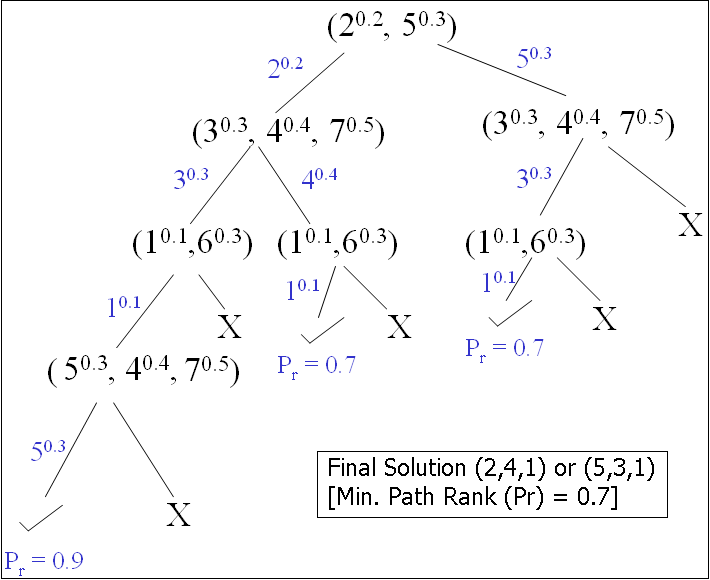
\includegraphics[width=90mm]{Figures/fig1.png}
\caption{Giải thuật HST được chỉnh sửa dựa theo thứ hạng của phát biểu \label{overflow}}
\end{figure}
\\\hspace*{.05\textwidth} Như được thể hiện trong hình, bằng cách chọn phát biểu có hạng thấp nhất trong từng tập trong khi xây cạnh của HST, giải thuật chỉ tạo ra 3 hitting sets, 2 trong số đó tối tiểu, trong khi hạn chế được một số lượng lớn số lần kiểm tra đường đi, (thể hiện bằng \xmark). Giải pháp sửa lỗi được tìm ra trong tập có $P_{r}$ nhỏ nhất là {2,4,1} hoặc {5,3,1}.
\hspace*{.05\textwidth} Tuy vậy, có một hạn chế khi sử dụng quy trình vừa nêu trên để tạo ra kế hoạch sửa lỗi, như phân tích tác động ngữ nghĩa của phát biểu chỉ được thực hiện ở cấp độ là một phát biểu đơn lẻ, trong khi một loạt tác động khác chưa được tính tới mỗi lần một HS được tìm thấy. Điều này có thể dẫn tới một giải pháp kém tối ưu. Ví dụ:
\begin{enumerate}
\item
DisjointClasses(Car Plane Ship)
EquivalentClass(FlyingCar (Car and Plane))
\item
\end{enumerate}
Trong ví dụ trên, bỏ \texttt{Plane} ra khỏi phát biểu (1) sẽ hạn chế mất mát về nghĩa hơn là xóa hết cả phát biểu (1), vì có thể disjoint giữa Car và Ship có thể được sử dụng đâu đó trong ontology mà chưa được tính đến.
\\\hspace*{.05\textwidth} Để khắc phục hạn chế này, một chỉnh sửa khác được đưa ra là cứ mỗi lần tìm ra hitting-set(HS), chúng ta sẽ tính lại thứ hạng của đường đi (path-rank) cho HS dựa trên một loạt tác động của các phát biểu trong hitting-set. Giải thuật bây giờ sẽ tìm được giải pháp tối thiểu được path-ranks mới.
\\
Trên đây là ý tưởng cơ bản của giải thuật HST, ngoài ta còn những mục về cải thiện các giải pháp sửa lỗi và gợi ý các phát biểu sửa lỗi xin đọc thêm ở [1].
\section{Ứng dụng giải thuật HST để tạo ra các giải thích}
Ngoài ứng dụng vừa được đề cập ở trên, giải thuật HST còn được dùng để tìm tất cả các giải thích cho một kết quả suy luận, đây cũng chính là chức năng chính của Axiom Pinpointing Service được đề cập lúc nãy.
 % Giải pháp sửa chữa ontology

\chapter{Kết luận}
Trong quá trình nghiên cứu về các nguyên nhân gây inconsistency trong ontology, chúng em đã tìm hiểu được nhiều giải pháp đã được nghiên cứu và ứng dụng. Chúng em cũng nắm được nguyên lý hoạt động những giải thuật và quy trình này như HST Explaination\textsuperscript{[9]} ,Blackbox Algorithm\textsuperscript{[8]} từ các tác giả của các bài báo [1],[8] và [9]. Hiện nay, những kỹ thuật trên đã được áp dụng trong nhiều ứng dụng thực tế mà cụ thể là thư viện OWL-API\textsuperscript{[2]} để tạo ra các giải thích cho một kết quả suy luận(entailment). Ngoài ra, chúng em cũng biết thêm được về khả năng sửa chữa lại các phát biểu unsatisfiable trong ontology là khả thi căn cứ vào bài báo [1]. Cuối cùng, chúng em nghĩ rằng việc tìm hiểu được các ứng dụng của các giải thuật Hitting Set Tree trong việc tìm ra phát biểu giải thích chính xác và ngắn gọn nhất hay tìm ra một tối tiểu trong các MUPS của ontology, sẽ rất hữu ích để ứng dụng vào việc đề xuất tập hợp các câu hỏi ngắn gọn và chính xác nhất từ tập hợp lớn các SWRL Rules trong ontology.
 

%\input{Chapters/Chapter4} % Experiment 1

%\input{Chapters/Chapter5} % Experiment 2

%\input{Chapters/Chapter6} % Results and Discussion

%\input{Chapters/Chapter7} % Conclusion

\chapter{Tài liệu tham khảo}
\begin{enumerate}
\item 
Aditya Kalyanpur, Bijan Parsia, Evren Sirin
, Bernardo Cuenca-Grau.Repairing Unsatisfiable Concepts in OWL Ontologies, 2007. Available online at \\ http://www.cs.ox.ac.uk/people/bernardo.cuencagrau/publications/repair.pdf
\item
The OWL API. The OWL API is a Java API for creating, parsing, manipulating and serialising OWL Ontologies. Available online at
https://github.com/owlcs/owlapi
\item
Pellet - OWL 2 Reasoner for Java.Pellet is an OWL 2 reasoner. Pellet provides standard and cutting-edge reasoning services for OWL ontologies. Available online at http://clarkparsia.com/pellet/
\item 
Robert Stevens. Ontogenesis, (I can’t get no) satisfiability Available online at http://ontogenesis.knowledgeblog.org/1329
\item
Samantha Bail.Ontogenesis, Common reasons for ontology inconsistency.Available online at http://ontogenesis.knowledgeblog.org/1343
\item 
S. Schlobach and R. Cornet. Non-standard reasoning services for the debugging of description logic terminologies. In Proceedings of IJCAI, 2003.
\item
R. Reiter. A theory of diagnosis from first principles. 1987. Artificial Intelligence
32:57-95.
\item
A. Kalyanpur, B. Parsia, B. Cuenca-Grau, and E. Sirin. Axiom pinpointing: Find-
ing (precise) justifications for arbitrary entailments in SHOIN (owl-dl). Technical
report, UMIACS, 2005-66, 2006. Technical Report
\item
Matthew Horridge, the University of Manchester. JUSTIFICATION BASED EXPLANATION IN ONTOLOGIES. Available online at: http://www.bcs.org/upload/pdf/dd-matthew-horridge.pdf
\end{enumerate}


 % Tài liệu tham khảo
%% ----------------------------------------------------------------
% Now begin the Appendices, including them as separate files

\addtocontents{toc}{\vspace{2em}} % Add a gap in the Contents, for aesthetics

\appendix % Cue to tell LaTeX that the following 'chapters' are Appendices

%\chapter{An Appendix}

Lorem ipsum dolor sit amet, consectetur adipiscing elit. Vivamus at pulvinar nisi. Phasellus hendrerit, diam placerat interdum iaculis, mauris justo cursus risus, in viverra purus eros at ligula. Ut metus justo, consequat a tristique posuere, laoreet nec nibh. Etiam et scelerisque mauris. Phasellus vel massa magna. Ut non neque id tortor pharetra bibendum vitae sit amet nisi. Duis nec quam quam, sed euismod justo. Pellentesque eu tellus vitae ante tempus malesuada. Nunc accumsan, quam in congue consequat, lectus lectus dapibus erat, id aliquet urna neque at massa. Nulla facilisi. Morbi ullamcorper eleifend posuere. Donec libero leo, faucibus nec bibendum at, mattis et urna. Proin consectetur, nunc ut imperdiet lobortis, magna neque tincidunt lectus, id iaculis nisi justo id nibh. Pellentesque vel sem in erat vulputate faucibus molestie ut lorem.

Quisque tristique urna in lorem laoreet at laoreet quam congue. Donec dolor turpis, blandit non imperdiet aliquet, blandit et felis. In lorem nisi, pretium sit amet vestibulum sed, tempus et sem. Proin non ante turpis. Nulla imperdiet fringilla convallis. Vivamus vel bibendum nisl. Pellentesque justo lectus, molestie vel luctus sed, lobortis in libero. Nulla facilisi. Aliquam erat volutpat. Suspendisse vitae nunc nunc. Sed aliquet est suscipit sapien rhoncus non adipiscing nibh consequat. Aliquam metus urna, faucibus eu vulputate non, luctus eu justo.

Donec urna leo, vulputate vitae porta eu, vehicula blandit libero. Phasellus eget massa et leo condimentum mollis. Nullam molestie, justo at pellentesque vulputate, sapien velit ornare diam, nec gravida lacus augue non diam. Integer mattis lacus id libero ultrices sit amet mollis neque molestie. Integer ut leo eget mi volutpat congue. Vivamus sodales, turpis id venenatis placerat, tellus purus adipiscing magna, eu aliquam nibh dolor id nibh. Pellentesque habitant morbi tristique senectus et netus et malesuada fames ac turpis egestas. Sed cursus convallis quam nec vehicula. Sed vulputate neque eget odio fringilla ac sodales urna feugiat.

Phasellus nisi quam, volutpat non ullamcorper eget, congue fringilla leo. Cras et erat et nibh placerat commodo id ornare est. Nulla facilisi. Aenean pulvinar scelerisque eros eget interdum. Nunc pulvinar magna ut felis varius in hendrerit dolor accumsan. Nunc pellentesque magna quis magna bibendum non laoreet erat tincidunt. Nulla facilisi.

Duis eget massa sem, gravida interdum ipsum. Nulla nunc nisl, hendrerit sit amet commodo vel, varius id tellus. Lorem ipsum dolor sit amet, consectetur adipiscing elit. Nunc ac dolor est. Suspendisse ultrices tincidunt metus eget accumsan. Nullam facilisis, justo vitae convallis sollicitudin, eros augue malesuada metus, nec sagittis diam nibh ut sapien. Duis blandit lectus vitae lorem aliquam nec euismod nisi volutpat. Vestibulum ornare dictum tortor, at faucibus justo tempor non. Nulla facilisi. Cras non massa nunc, eget euismod purus. Nunc metus ipsum, euismod a consectetur vel, hendrerit nec nunc.	% Appendix Title

%\input{Appendices/AppendixB} % Appendix Title

%\input{Appendices/AppendixC} % Appendix Title

\addtocontents{toc}{\vspace{2em}}  % Add a gap in the Contents, for aesthetics
\backmatter

%% ----------------------------------------------------------------
\label{Bibliography}
\lhead{\emph{Bibliography}}  % Change the left side page header to "Bibliography"
\bibliographystyle{unsrtnat}  % Use the "unsrtnat" BibTeX style for formatting the Bibliography
\bibliography{Bibliography}  % The references (bibliography) information are stored in the file named "Bibliography.bib"

\end{document}  % The End
%% ----------------------------------------------------------------